% Candidate source: src-cb0092e0533abc5b37a4e6843ba9688dfd851d0597a8dd9d44a827bd35e58290
% Source PDF SHA-256: 4ffc26d1ee893834e7cdf6a1b6ab3385fb97dd791d838d2630538461026ca7ad
% PDF page 2 (printed page 201), question 20.
% Redraw follows visible relations; point placement is schematic, not a scale claim.
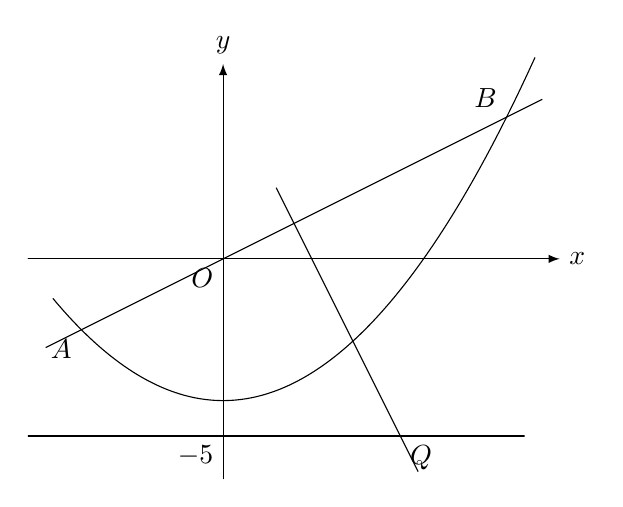
\begin{tikzpicture}[line cap=round,line join=round,>=latex,x=0.45cm,y=0.45cm]
  % Axes
  \draw[->] (-5.5,0) -- (9.5,0) node[right] {$x$};
  \draw[->] (0,-6.2) -- (0,5.5) node[above] {$y$};
  \node[below left] at (0,0) {$O$};

  % Horizontal line y = -5
  \draw (-5.5,-5) -- (8.5,-5);
  \node[below left] at (0,-5) {$-5$};

  % Parabola y = 1/8 x^2 - 4
  \draw[smooth,samples=100,domain=-4.8:8.8] plot (\x,{0.125*\x*\x - 4});

  % Line y = 1/2 x and chord AB
  \coordinate (A) at (-4,-2);
  \coordinate (B) at (8,4);
  \draw (-5.0,-2.5) -- (9.0,4.5);

  % Perpendicular bisector of AB intersecting y = -5 at Q(5, -5)
  \coordinate (M) at (2,1);
  \coordinate (Q) at (5,-5);
  \draw (1.5,2.0) -- (5.5,-6.0);

  % Nodes
  \node[below left] at (A) {$A$};
  \node[above left] at (B) {$B$};
  \node[below right] at (Q) {$Q$};
\end{tikzpicture}
